%% Supplementary Material — Paper A (JNCA), compiled separately from main.tex.
%% Tables S1–S4 and Figures S1–S5 referenced from the main text as
%% "Supplementary Tab.~S<n>" / "Supplementary Fig.~S<n>".
\documentclass[a4paper,11pt]{article}
\usepackage[utf8]{inputenc}
\usepackage[T1]{fontenc}
\usepackage[english]{babel}
\usepackage[margin=2.5cm]{geometry}
\usepackage{graphicx}
\usepackage{booktabs}
\usepackage{amsmath}
\graphicspath{{figures/}}

\renewcommand{\thetable}{S\arabic{table}}
\renewcommand{\thefigure}{S\arabic{figure}}

\title{Supplementary Material for\\
\emph{Lateral Phishing as a Violation of the Organizational Communication Graph:\\
Cascade Dynamics and Leak-Aware Evaluation}}
\author{Kamil Warpechowski \and Bogdan Ksi\k{e}\.zopolski}
\date{}

\begin{document}
\maketitle

\noindent This supplement contains secondary tables and figures referenced from the main text.
All values are produced by the reproducibility package (\texttt{code/results/*.csv}); none are new
experiments.

\section*{S1. Detector hyperparameters}

\begin{table}[h]\centering\small
\begin{tabular}{ll}
\toprule
Model / component & Hyperparameters (fixed, without tuning) \\
\midrule
GNN (static / TGN-lite / TGAT-lite) & $\mathrm{DIM}{=}24$; TGAT: $t_{\dim}{=}8$; $100$~epochs; \\
                                       & Adam $\mathrm{lr}{=}0.01$, $\mathrm{wd}{=}5\!\cdot\!10^{-4}$; dropout $0.2$ \\
GNN classifier head           & MLP, $48$ hidden units \\
Tabular detectors (LightGBM)      & $\mathrm{n\_estimators}{=}200$--$250$, $\mathrm{seed}{=}42$, \\
                                       & $\mathrm{num\_leaves}{=}31$, $\mathrm{lr}{=}0.1$ \\
volumetric / path-based (LightGBM) & $\mathrm{n\_estimators}{=}200$, $\mathrm{seed}{=}42$; context window $W{=}2$~buckets \\
\bottomrule
\end{tabular}
\caption{Detector hyperparameters: fixed \emph{uniformly} for all models of a given family, framework
defaults or lightly chosen, without grid search.}
\label{stab:hparams}
\end{table}

\section*{S2. Cascade detectors and the cascade-model sweep}

\begin{figure}[h]\centering
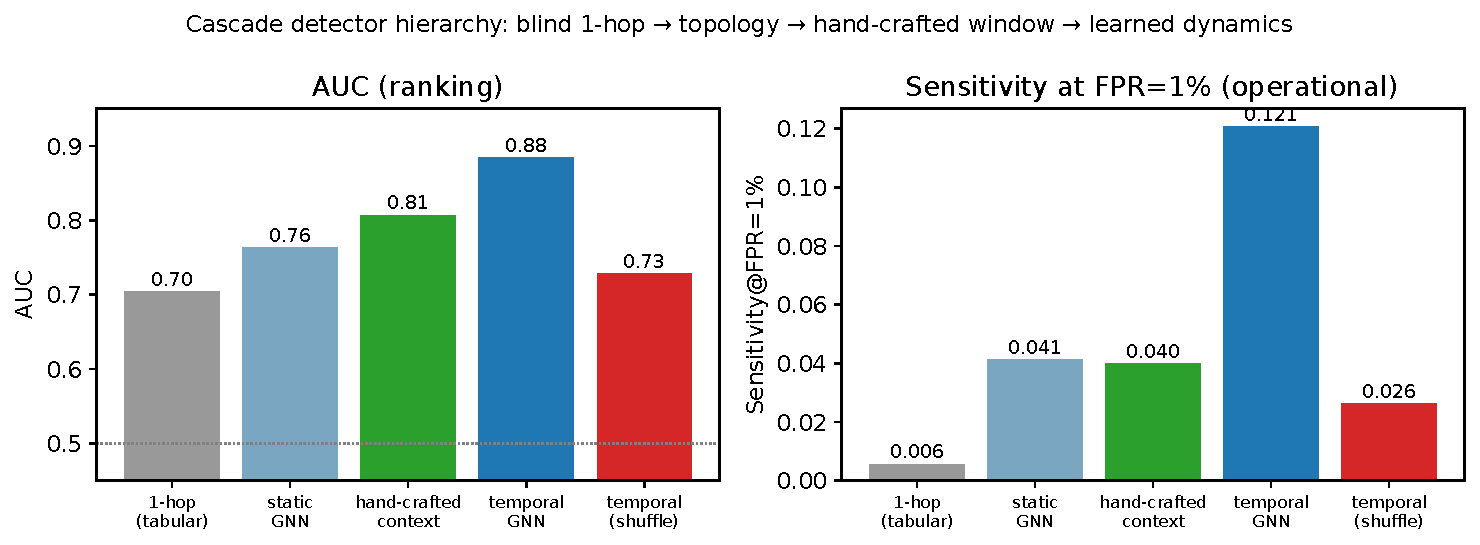
\includegraphics[width=\linewidth]{fig_cascade_detectors.pdf}
\caption{Detector hierarchy on AUC (left) and sensitivity@FPR1\% (right); values as in the cascade-detector
table of the main text. The temporal GNN dominates; time shuffling (red) levels it with the static GNN.}
\label{sfig:detectors}
\end{figure}

\begin{table}[h]\centering\small
\begin{tabular}{l ccccccc}
\toprule
$p_\mathrm{inf}$ & $0.05$ & $0.1$ & $0.2$ & $0.3$ & $0.5$ & $0.7$ & $0.9$ \\
\midrule
1-hop        & $0.60$ & $0.56$ & $0.59$ & $0.60$ & $0.68$ & $0.73$ & $0.79$ \\
manual & $0.75$ & $0.77$ & $0.77$ & $0.79$ & $0.79$ & $0.81$ & $0.85$ \\
temporal   & $\mathbf{0.97}$ & $\mathbf{0.95}$ & $\mathbf{0.90}$ & $\mathbf{0.87}$ & $\mathbf{0.87}$ & $\mathbf{0.89}$ & $\mathbf{0.92}$ \\
\bottomrule
\end{tabular}
\caption{Cascade model sweep (AUC, depth~$4$, $8$~seeds): the hierarchy holds across the whole range of the
infection probability, and the receiving-side signal does not vanish at a realistically low
$p_\mathrm{inf}$.}
\label{stab:pinf}
\end{table}

\clearpage
\section*{S3. Inductive validation under increasing scale}

\begin{table}[h]\centering
\begin{tabular}{lcccc}
\toprule
& \multicolumn{2}{c}{AUC} & \multicolumn{2}{c}{sensitivity@FPR$1\%$} \\
\cmidrule(lr){2-3}\cmidrule(lr){4-5}
Organizations & temp. & manual & temp. & manual \\
\midrule
$19$  & $0.76$ & $0.75$ & $\mathbf{0.062}$ & $0.027$ \\
$30$  & $0.69$ & $0.75$ & $\mathbf{0.041}$ & $0.025$ \\
$200$ & $0.78$ & $0.81$ & $\mathbf{0.076}$ & $0.042$ \\
\bottomrule
\end{tabular}
\caption{Inductive validation on unseen organizations ($19$~organizations: $5$~seeds; $30$ and
$200$~organizations: $3$~seeds): the temporal detector's operational advantage over the hand-crafted context
holds on companies never seen in training at every scale ($2.3\times$, $1.7\times$, $1.8\times$), while its
AUC does not lead at the two larger scales.}
\label{stab:scale}
\end{table}

\begin{figure}[h]\centering
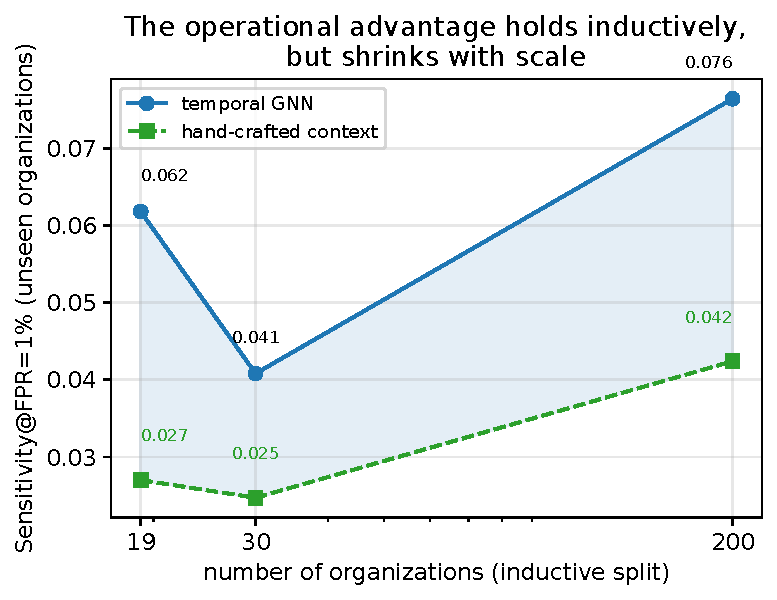
\includegraphics[width=0.62\linewidth]{fig_cascade_scale.pdf}
\caption{Inductive validation: sensitivity@FPR1\% on unseen organizations against the number of companies
(values as in Tab.~S3). The advantage holds inductively at every scale ($2.3\times$, $1.7\times$, $1.8\times$).}
\label{sfig:scale}
\end{figure}

\clearpage
\section*{S4. Replication on real topologies}

\begin{figure}[h]\centering
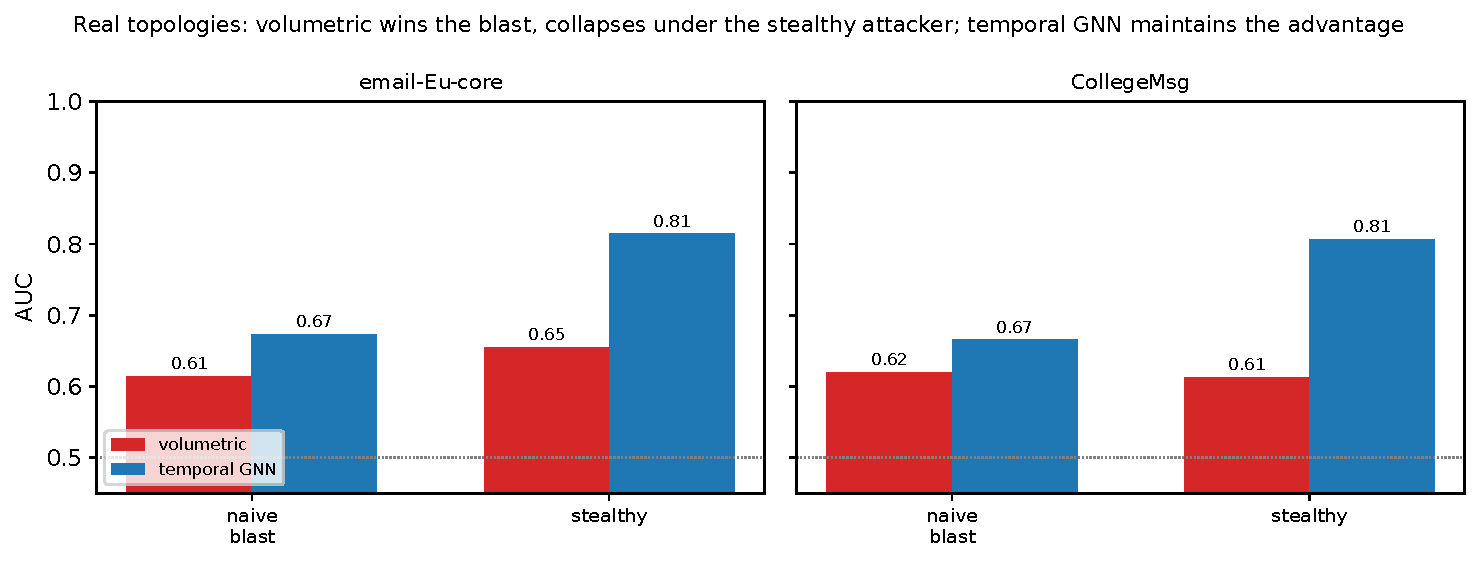
\includegraphics[width=\linewidth]{fig_cascade_realgraphs.pdf}
\caption{Two real topologies (\texttt{email-Eu-core}, \texttt{CollegeMsg}). The volumetric detector is
weak in both regimes; the temporal GNN (blue) is ahead in both and its advantage is largest under the
stealthy attack, where the volumetric operating point collapses. Values as in block~(b) of the real-graph table of the main text.}
\label{sfig:realgraphs}
\end{figure}

\begin{figure}[h]\centering
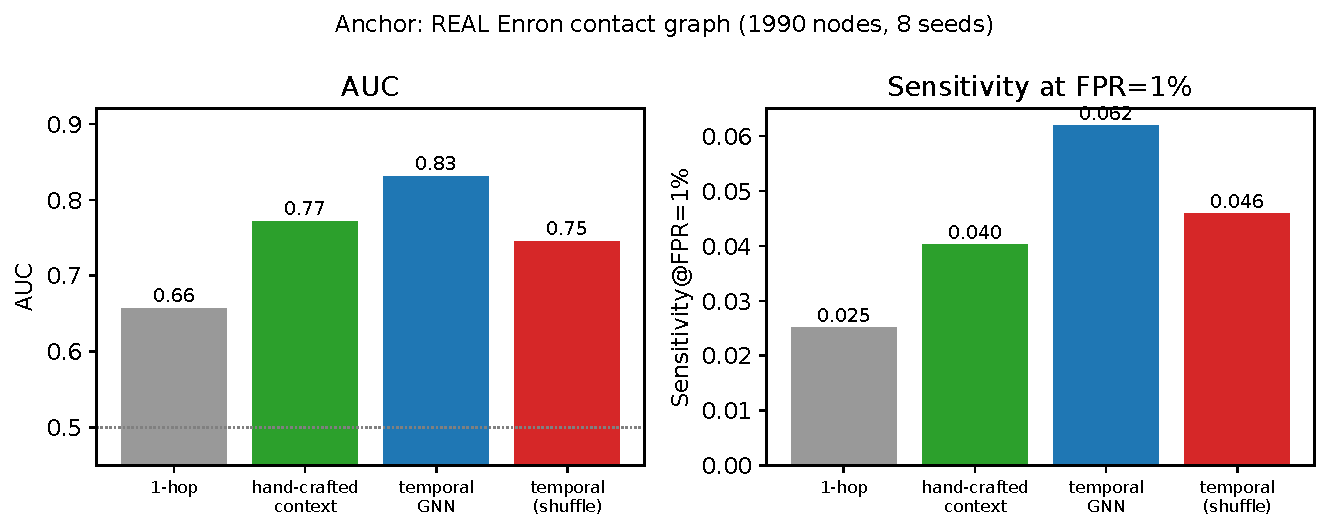
\includegraphics[width=\linewidth]{fig_cascade_enron.pdf}
\caption{The cascade invariant on Enron (values as in block~(a) of the real-graph table of the main text):
the same hierarchy as on the case-study graph (1-hop $<$ hand-crafted context $<$ temporal GNN), with the
time shuffle bringing the temporal detector back close to the hand-crafted result.}
\label{sfig:enroncasc}
\end{figure}

\clearpage
\section*{S5. Rigor: label noise and the sensitivity--FPR curve}

\begin{table}[h]\centering
\begin{tabular}{lcccc}
\toprule
Label noise & vol. & path & manual & temp. \\
\midrule
$0\%$   & $0.60$ & $0.66$ & $0.67$ & $\mathbf{0.73}$ \\
$5\%$   & $0.60$ & $0.66$ & $0.66$ & $\mathbf{0.70}$ \\
$10\%$  & $0.60$ & $0.65$ & $0.65$ & $\mathbf{0.66}$ \\
$20\%$  & $0.59$ & $\mathbf{0.63}$ & $0.61$ & $0.60$ \\
\bottomrule
\end{tabular}
\caption{Audit of noisy training labels (AUC; stealthy attack at $K{=}3$ in the second harness
(\texttt{cascadebench}, $600$-account organization; the baseline table of the main text);
$20$~seeds): the learned temporal model
degrades fastest ($0.73\!\to\!0.60$), so its advantage shrinks under realistic label noise.}
\label{stab:labelnoise}
\end{table}

\begin{figure}[h]\centering
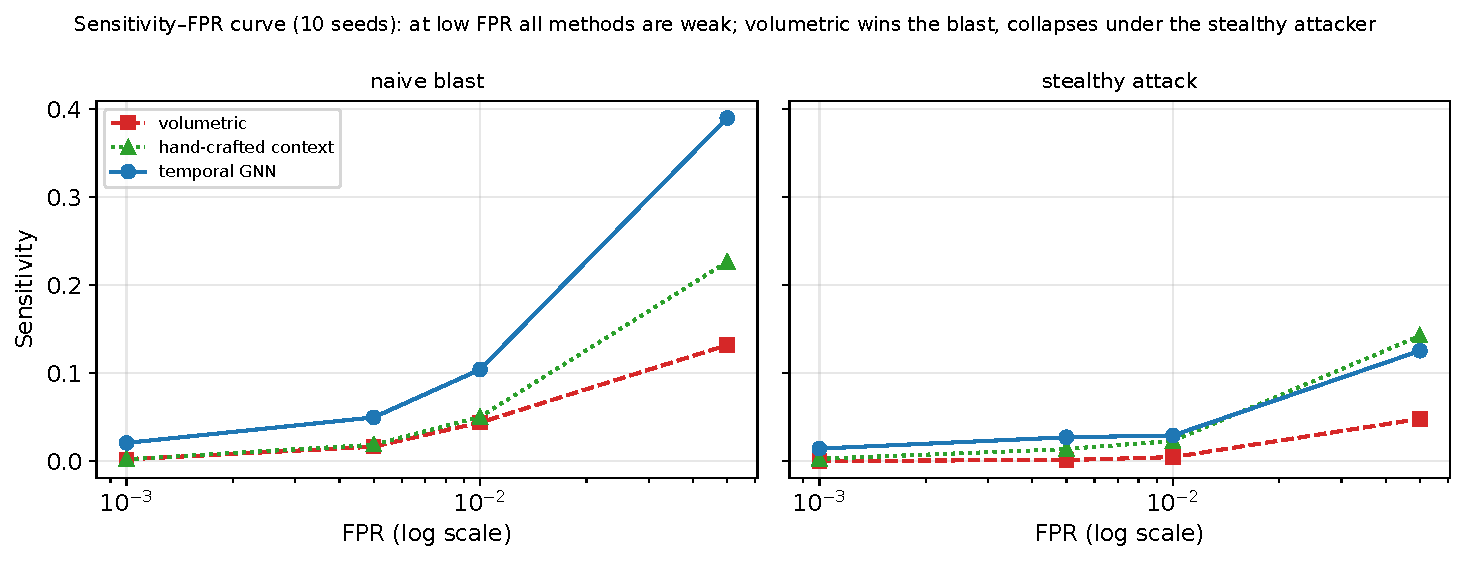
\includegraphics[width=\linewidth]{fig_cascade_fpr.pdf}
\caption{Sensitivity--FPR curve ($10$~seeds). At low FPR all methods are weak; the volume detector dominates
the blast and breaks down under the stealthy attack, where the receiving-side signal degrades less.}
\label{sfig:fpr}
\end{figure}

\clearpage
\section*{S6. Feature specification of every detector}

\noindent All tabular detectors use the same learner (LightGBM, $200$--$250$~trees as in Tab.~S1, seed~$42$); they differ only in
their features. Time is divided into buckets $b$; the context window is $W{=}2$ buckets. $\mathcal{N}(v)$ is
the set of contacts of $v$ in the communication graph; $\mathrm{recv}(b)$ and $\mathrm{sent}(b)$ are the sets
of accounts that received, respectively sent, mail in bucket $b$; $\mathrm{rhythm}(s,b)$ is the
temporal-consistency bit $tc$. The two experiment harnesses of the package (\texttt{experiments/} for the
cascade, stealth, scale, and real-graph tables; \texttt{cascadebench/} for the baseline, label-noise, and
headline-contrast tables) implement identical feature definitions.

\begin{itemize}
  \item \textbf{1-hop (tabular).} For event $s\!\to\!v$ in bucket $b$: $\mathbf{1}[s\in\mathcal{N}(v)]$,
  $\mathrm{rhythm}(s,b)$, $|\mathcal{N}(v)|$, $|\mathcal{N}(s)|$.
  \item \textbf{Hand-crafted cascade context.} The 1-hop features plus three receiving-side statistics,
  all computed from strictly past buckets ($\le b-1$):
  \emph{burst} $=|(\mathcal{N}(v)\setminus\{s\})\cap\bigcup_{b'=b-W}^{b-1}\mathrm{recv}(b')|/|\mathcal{N}(v)|$
  (how many of the victim's other contacts were hit within the past window); \emph{freshness}
  $=\mathbf{1}[s\in\bigcup_{b'=b-W}^{b-1}\mathrm{recv}(b')]$ (the sender was itself hit just before);
  \emph{propagation} $=|(\mathcal{N}(v)\setminus\{s\})\cap\bigcup_{b'=b-W}^{b-1}\mathrm{sent}(b')|/|\mathcal{N}(v)|$
  (how many of the victim's other contacts are themselves sending).
  \item \textbf{Volumetric baseline (inspired by COMPA).} Three per-event deviations of the sender from its own
  profile, computed from strictly past buckets ($<b$): recipient novelty $1/(1+\#\{s\!\to\!v \text{ before } b\})$, time novelty
  $1/(1+\#\{\text{events of } s \text{ in buckets} < b\})$, and sender activity $\#\{\text{events of } s \text{ before } b\}$. COMPA
  itself detects compromised accounts on social networks by comparing each new message with a behavioral
  profile of the account (time of day, source, language, links, topics); we transfer only its
  per-sender-deviation idea to email headers, restricted to volume and timing.
  \item \textbf{Path-based baseline (inspired by Hopper).} \emph{Precursor} $=\mathbf{1}[s\in\bigcup_{b'=b-W}^{b-1}\mathrm{recv}(b')]$
  (the sender was reached just before, i.e.\ is part of a chain); \emph{momentum} $=$ number of distinct
  targets of $s$ in buckets $[b-W,b-1]$; \emph{rare target} $=1/(1+\text{popularity of } v \text{ as a recipient before } b)$;
  \emph{unexplained} $=1-\mathrm{rhythm}(s,b)$; and the conjunction $\text{precursor}\times\text{unexplained}$.
  All windows are strictly past, matching the temporal model's memory: an earlier draft of the package
  defined momentum over $[b,b+W]$ (future buckets) and the volumetric counters over the full stream; both
  were look-ahead leaks, and every experiment was re-run after the fix.
  Hopper itself detects lateral movement in enterprise networks from authentication logs, by reconstructing
  login paths between machines and flagging paths with no benign explanation; it does not process email. We
  transfer its causal-path idea (a precursor that explains the hop, and a rare target) to the email
  communication graph.
  \item \textbf{Static GNN.} Node features $X=\log(1+[\,|\mathcal{N}(u)|,\ \text{in-degree}(u),\ \text{out-degree}(u)\,])$
  (three dimensions, the stream degrees computed from the \emph{training} split only), projected to $\mathrm{DIM}{=}24$ and propagated through two
  layers with the normalized adjacency (Eq.~(1) of the main text). The head $g$ is an MLP with $48$ hidden
  units and dropout $0.2$ over $[Z_s, Z_v, Z_s\!\odot\!Z_v, x_{sv}]$, where $x_{sv}$ is the 1-hop feature vector
  of the event.
  \item \textbf{Temporal GNN (TGN-lite).} Same node features and $x_{sv}$; a memory of dimension $24$ per node,
  updated bucket by bucket with a GRU cell from the mean of the messages $\sigma(W_m m_u^{(b-1)})$ of the
  senders that reached the node in bucket $b$ (Eq.~(3)); an event of bucket $b$ is scored from the memories of
  bucket $b-1$ (Eq.~(2)) by the same head as the static GNN. TGAT-lite replaces the mean pooling by attention
  with an $8$-dimensional time encoding. Training: Adam ($\mathrm{lr}{=}0.01$, weight decay $5\cdot10^{-4}$),
  $100$~epochs, binary cross-entropy.
\end{itemize}

\clearpage
\section*{S7. Seed counts per experiment}

\begin{table}[h]\centering\small
\begin{tabular}{llc}
\toprule
Experiment & Table / figure & Seeds \\
\midrule
Detector hierarchy (case study) & main-text detector table, Fig.~S1 & $5$ \\
Library TGN (extra row) & main-text detector table & $3$ \\
Architecture robustness (TGN-lite / TGAT-lite) & Sec.~S1 & $5$ \\
Stealthy attacker sweep & main-text stealth table, Fig.~S2 & $20$ \\
Baselines (a) stealth / (b) surgical & main-text baseline table & $20$ \\
Headline contrasts (Wilcoxon, Cliff's $\delta$) & main-text rigor section & $20$ \\
Label-noise audit & Tab.~S4 & $20$ \\
Static-blindness audit (compromised senders) & --- & $20$ \\
Cascade-model sweep & Tab.~S2 & $8$ \\
Inductive validation ($19$ / $30$ / $200$ org.) & Tab.~S3, Fig.~S3 & $5$ / $3$ / $3$ \\
Sensitivity--FPR curve & Fig.~S5 & $10$ \\
Enron cascade & main-text real-graph table (a), Fig.~S4 & $8$ \\
SNAP graphs (\texttt{email-Eu-core}, \texttt{CollegeMsg}) & main-text real-graph table (b) & $3$ \\
\bottomrule
\end{tabular}
\caption{Number of random seeds behind every reported aggregate. The stealthy, baseline,
label-noise, and contrast experiments use $20$~seeds; the detector hierarchy and architecture checks
$5$; real-graph replications use $8$ (Enron) and $3$ (SNAP), and are reported as directional
confirmations.}
\label{stab:seeds}
\end{table}

\end{document}
